\documentclass[13pt,a4paper]{extarticle}
\usepackage[utf8]{inputenc}
\usepackage[utf8]{vietnam} %Bien dich duoc tieng Viet
\usepackage{amsmath,amsfonts,amssymb} %Font toan
\usepackage{type1cm}
\usepackage{times}
\usepackage{graphicx}
\graphicspath{ {images06/} }
\usepackage{enumerate}
\usepackage{comment}
\usepackage{multicol}
\usepackage{multirow}
%\usepackage[unicode]{hyperref} %Tu dong tao bookmark
\usepackage[unicode, hidelinks=true]{hyperref}
\usepackage{indentfirst} %Thut vao dau dong o tat ca cac doan
\usepackage{listings} %Dinh dang code
\usepackage{color} %Mau sac
\usepackage[left=2.5cm,right=2.5cm,top=2.5cm,bottom=2.5cm]{geometry} %Canh lề trái - phải - trên - dưới cho tài liệu
\usepackage{longtable}
\renewcommand{\arraystretch}{1.3}

\begin{document}
\pagenumbering{gobble}
\title{\Large{\textbf{BÀI CHUẨN BỊ THỰC TẬP ĐIỆN CÔNG NGHIỆP}}\\\vspace{1cm}\textbf{Bài 6}\\\vspace{.5cm}\textbf{VẬN HÀNH VÀ ĐIỀU KHIỂN HỆ THỐNG BƠM NƯỚC TỰ ĐỘNG TRONG CÔNG NGHIỆP}}
\date{Ngày 09 tháng 06 năm 2016}
%\date{\today}
\author{GVHD: Võ Minh Thiện \vspace{.6cm}\\  Nhóm SVTH: Nhóm 2 -- Tiểu nhóm 1: Thi Minh Nhựt}
\maketitle
\tableofcontents
\newpage
\pagenumbering{arabic}
\setcounter{page}{1}
\section{Điều khiển trực tiếp bằng bộ khởi động từ}
Lắp mạch động lực và mạch điều khiển như \ref{Fig:relay-dien-cuc}.
\begin{figure}[!h]
\begin{center}
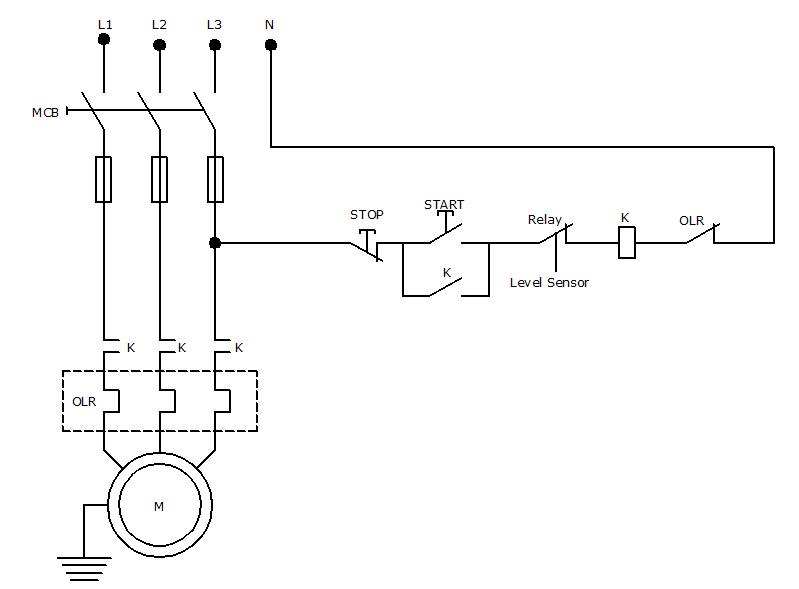
\includegraphics[scale=.7]{1}
\end{center}
\caption{Mạch động lực và mạch điều khiển sử dụng Relay điện cực}
\label{Fig:relay-dien-cuc}
\end{figure}

\begin{list}{--}{}
\item Khi sử dụng công tắc cho các nút STOP, START thì không cần phải sử dụng thêm tiếp điểm thường mở NO của contactor để duy trì mạch.
\item Vận hành mạch điều khiển, xác định điện áp nguồn điện.
\item Vận hành: Nhấn nút START để chạy mô hình. Nhấn nút STOP để dừng mô hình.
\item Vận hành mạch động lực: Nối các điện cực của cảm biến mực chất lỏng đến các điểm $E1,E2,E3$. Cấp nguồn $220V$ cho khối cảm biến hoạt động.
\end{list}
\paragraph{Nguyên lý hoạt động}
\begin{list}{--}{}
\item Relay điện cực có 3 thanh điện cực nhận biết mực chất lỏng ở các mức: thấp, trung bình và cao.
\item Khi mực chất lỏng ở đến thanh điện cực ở mức cao thì relay điện cực sẽ mở ra, dừng bơm nước.
\item Khi mực nước ở mức thấp thì cho bơm nước tự động trở lại nhờ vào cảm biến chất lỏng (các thanh điện cực).
\end{list}
\section{Điều khiển bằng bộ biến tần}
\begin{list}{--}{}
\item Lắp mạch điều khiển như hình \ref{Fig:bien-tan}.
\begin{figure}[!h]
\begin{center}
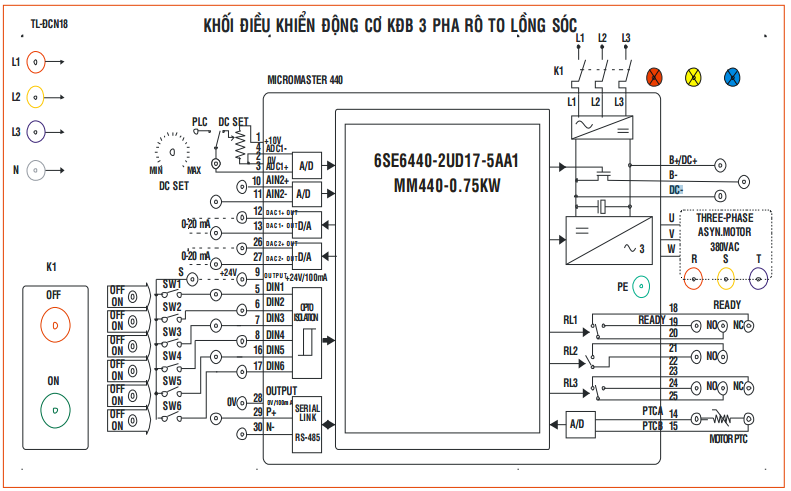
\includegraphics[scale=.7]{2}
\end{center}
\caption{Mạch điều khiển bơm nước sử dụng biến tần}
\label{Fig:bien-tan}
\end{figure}
\item Cấp nguồn 3 pha vào các chốt $L1,L2,L3,N$. Cấp nguồn cho động cơ vào các chốt $R,S,T$.
\item Sử dụng tiếp điểm thường đóng của relay điện cực thay thế cho công tắc như hình \ref{Fig:NC-relay}.
\begin{figure}[!h]
\begin{center}
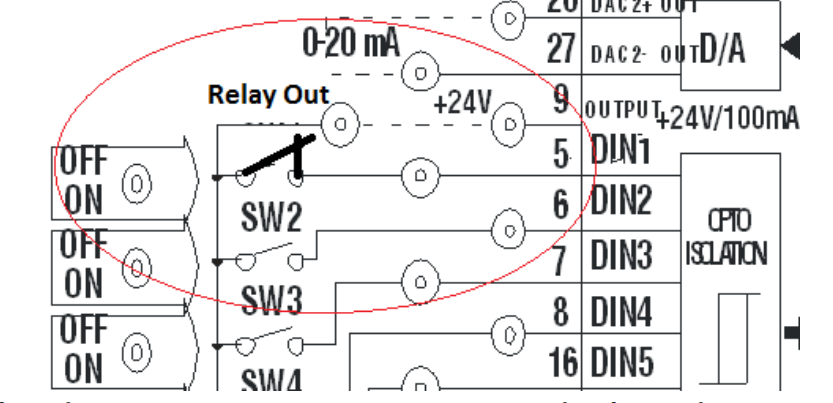
\includegraphics[scale=.4]{3}
\end{center}
\caption{Thay công tắc SW1 bằng tiếp điểm NC của relay điện cực}
\label{Fig:NC-relay}
\end{figure}
\item Vận hành mạch điều khiển kết hợp với biến tần.
\begin{list}{+}{}
\item Kết nối các thanh điện cực đến $E1,E2,E3$.
\item Cấp nguồn 220V cho khối cảm biến.
\item Thiết lập ở chế độ cao $E1$ thì ngắt, mức thấp $E3$ thì bơm.
\item Thiết lập các thông số của biến tần phù hợp với motor:
\begin{center}
\begin{tabular}{|c|l|}\hline
Mã & Ý nghĩa\\ \hline
$P0100 = 0$ & Tần số $50Hz$, công suất kW (0)\\ \hline
$P0300 = 1$ & Động cơ không đồng bộ \\ \hline
$P0301 = 380$ & Điện áp làm việc $380V$\\ \hline
$P0305 = I$ & Dòng làm việc \\ \hline
$P0307 = P$ & Công suất định danh của động cơ\\ \hline
$P0308 = \cos \varphi$ & Hệ số công suất \\ \hline
$P0310 = f$ & Tần số làm việc \\ \hline
$P0311 = n$ & Tốc độ làm việc của động cơ \\ \hline
\end{tabular}
\end{center}
\item Đặt $P3900 = 1$ để nhớ lại các giá trị cài đặt. Đặt $P0004 = 0 $ và $P0010 = 0$ để biến tần sẵn sàn làm việc.
\end{list}
\item Điều khiển bơm tự động:
\begin{list}{+}{}
\item Nhấn nút ON cấp nguồn cho biến tần hoạt động. 
\item Đặt công tắc $Mode = Man$.
\item Thiết lặp các thông số cho biến tần:
\begin{center}
\begin{tabular}{|c|l|}\hline
Mã & Ý nghĩa\\ \hline
$P0700 = 2$ & Chọn nguồn từ Terminal\\ \hline
$P1000 = 1$ & Đặt giá trị tần số kiểu tương tự \\ \hline
$P0701 = 380$ & Sử dụng chức năng của chân DIN1\\ \hline
$P1080 = f_{min}$ & Tần số cực tiểu \\ \hline
$P1082 = f_{max}$ & Tần số cực đại nhỏ hơn tần số định danh của động cơ\\ \hline
\end{tabular}
\end{center}
\end{list}
\item Vận hành hệ thống: nhấn nút ON để vận hành và nhấn nút STOP để dừng.
\end{list}
\end{document}